\newpage

\section{Проектирование системы}

\subsection{Проектирование архитектуры ПО (модули)}

\subsubsection*{Иерархия модулей и подмодулей разрабатываемой программы для frontend}

Информационная система включает в себя следующие модули на frontend:

\begin{itemize}
    \item \textbf{Error404} - модуль не найденной страницы
    \item \textbf{Singin} - модуль авторизации
    \item \textbf{Singout} - модуль выхода
    \item \textbf{Product} - модуль для продукта
    \item \textbf{Product/add} - модуль, реализующий добавление новых записей в базу данных;
    \item \textbf{Product/get} - модуль организации локальной базы данных с выводом информации о товарах;
    \item \textbf{Product/get/delete} - модуль удаления записи из локальной базы данных;
    \item \textbf{Product/edit} - модуль, осуществляющий изменение записи;
    \item \textbf{Product/download\_json} - модуль, осуществляющий сохранение данных в JSON;
    \item \textbf{Product/download\_csv} - модуль, осуществляющий сохранение данных в CSV;
    \item \textbf{Product/open} - модуль, осуществляющий открытие файла JSON.
    \item \textbf{Nav} - модуль меню
\end{itemize}

Схема frontend модулей изображена на
\textbf{рис. \ref{fig:gpi_frontend_modules} (стр. \pageref{fig:gpi_frontend_modules})}.

\begin{figure}[!hp]
    \centering
    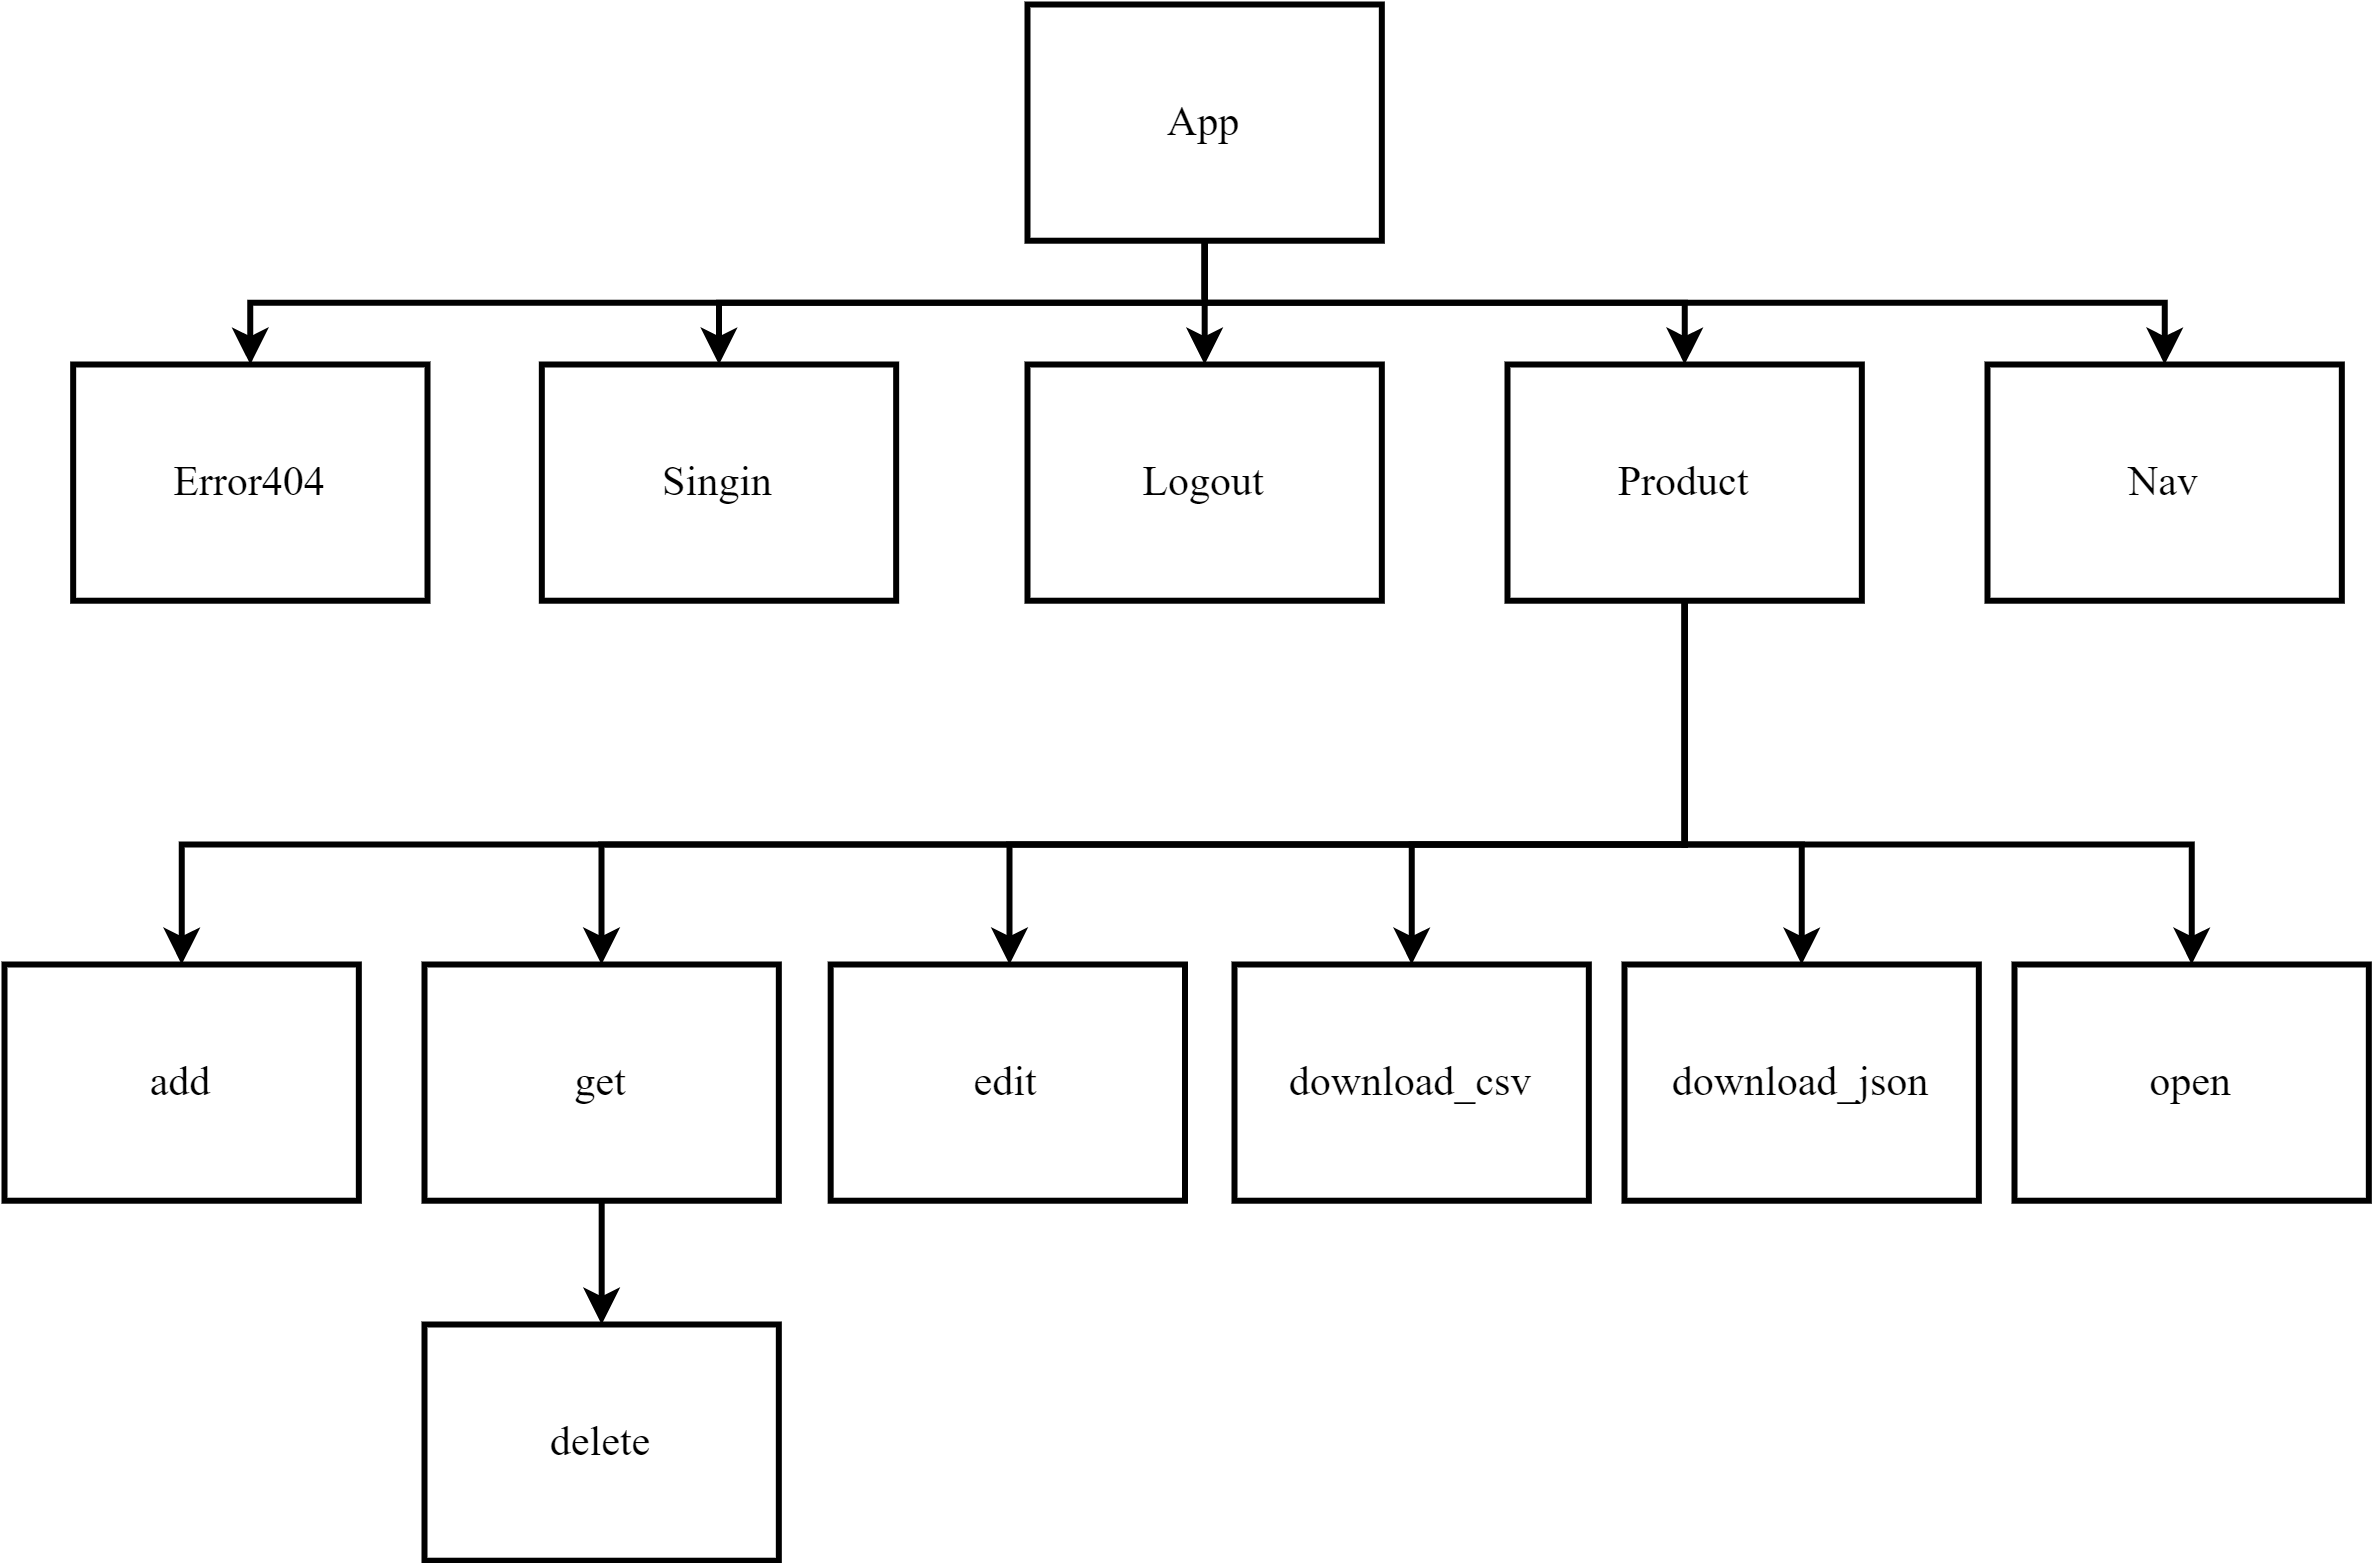
\includegraphics[width=16cm]
        {_assets/gpi_frontend_modules.png}
    \caption{Модули и подмодули для frontend}
    \label{fig:gpi_frontend_modules}
\end{figure}

\subsubsection*{Иерархия модулей и подмодулей разрабатываемой программы для backend}

Информационная система включает в себя следующие модули на backend:

\begin{itemize}
    \item \textbf{products/add} - модуль добавления элементов в базу данных;
    \item \textbf{products/get} - модуль вывода элементов сортированных, инвертированных или по ID;
    \item \textbf{products/edit} - модуль редактирования элемента по ID;
    \item \textbf{products/delete} - модуль удаления элемента по ID.
    \item \textbf{singin} - модуль авторизации;
\end{itemize}

Схема backend модулей изображена на
\textbf{рис. \ref{fig:gpi_backend_modules} (стр. \pageref{fig:gpi_backend_modules})}.

\begin{figure}[!hp]
    \centering
    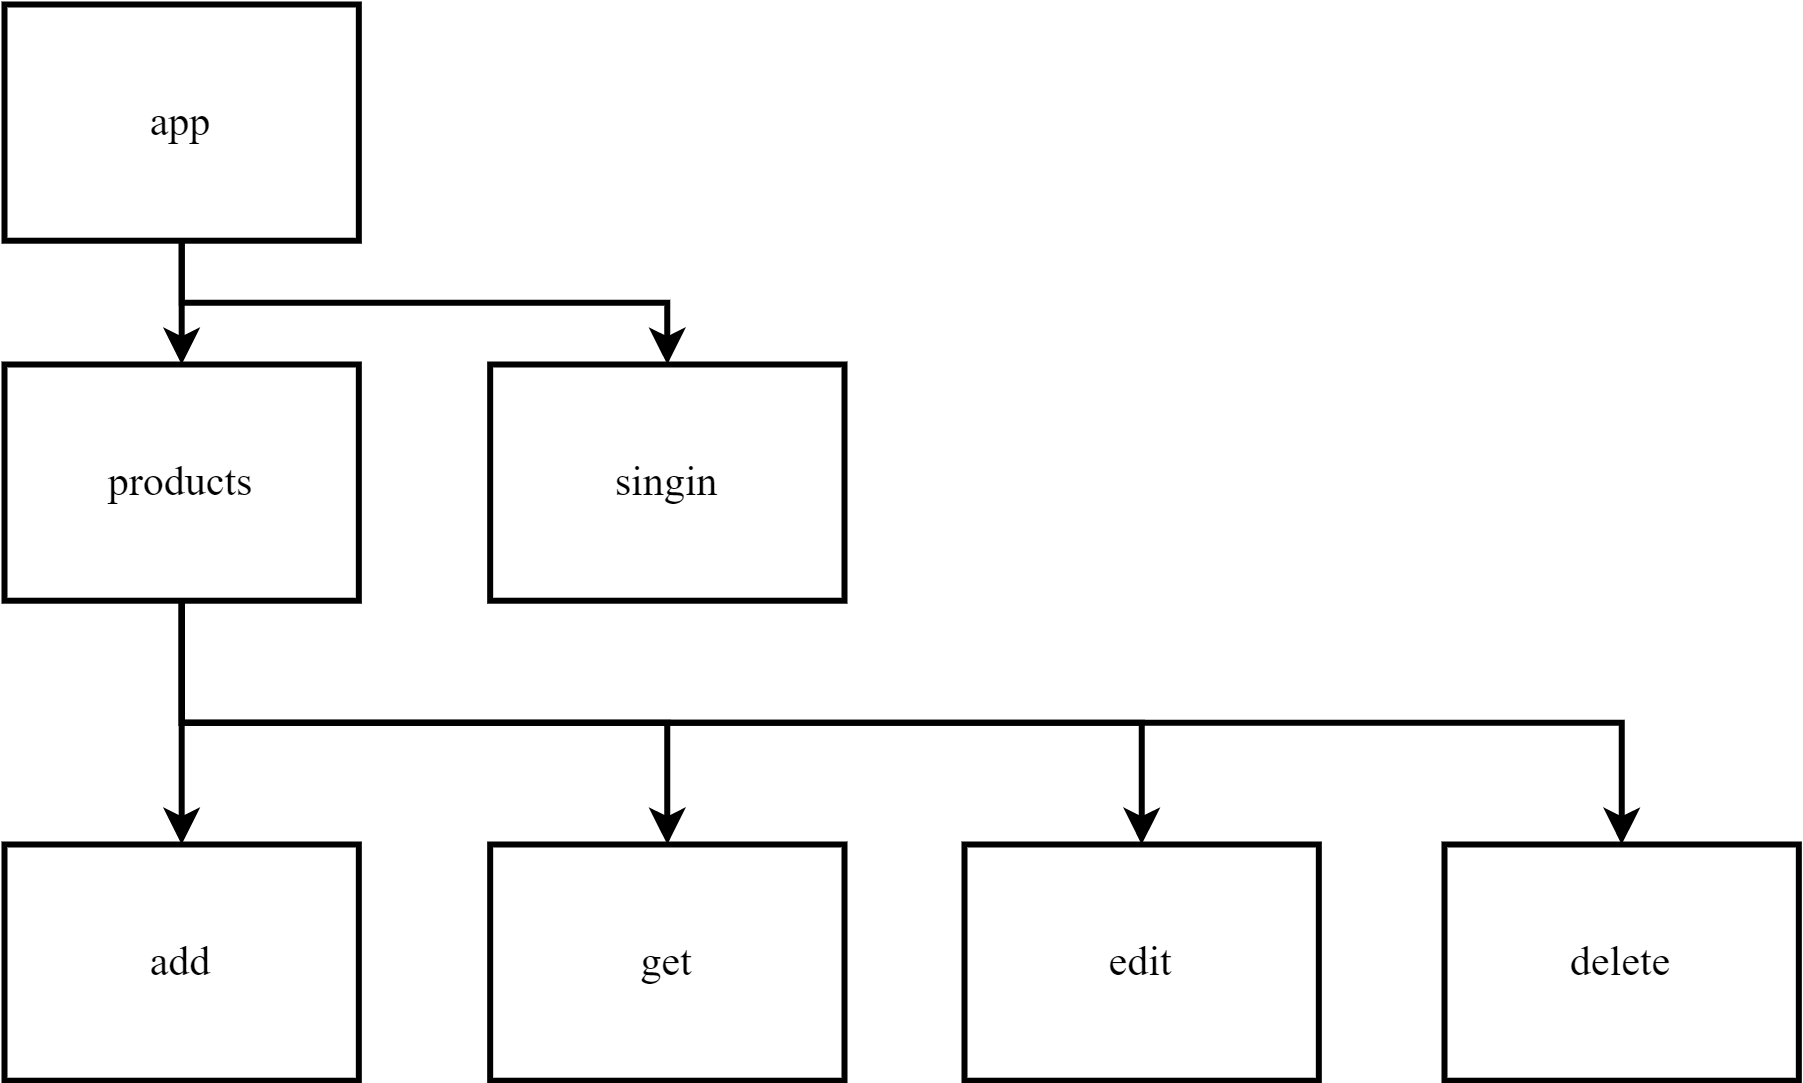
\includegraphics[width=16cm]
        {_assets/gpi_backend_modules.png}
    \caption{Модули и подмодули для backend}
    \label{fig:gpi_backend_modules}
\end{figure}

\newpage

\subsection{Проектирование UI (макеты)}

Макет меню для компьютера изображен на
\textbf{рис.~\ref{fig:gpi_ui_menu}~(стр.~\pageref{fig:gpi_ui_menu})}.

\begin{figure}[!hp]
    \centering
    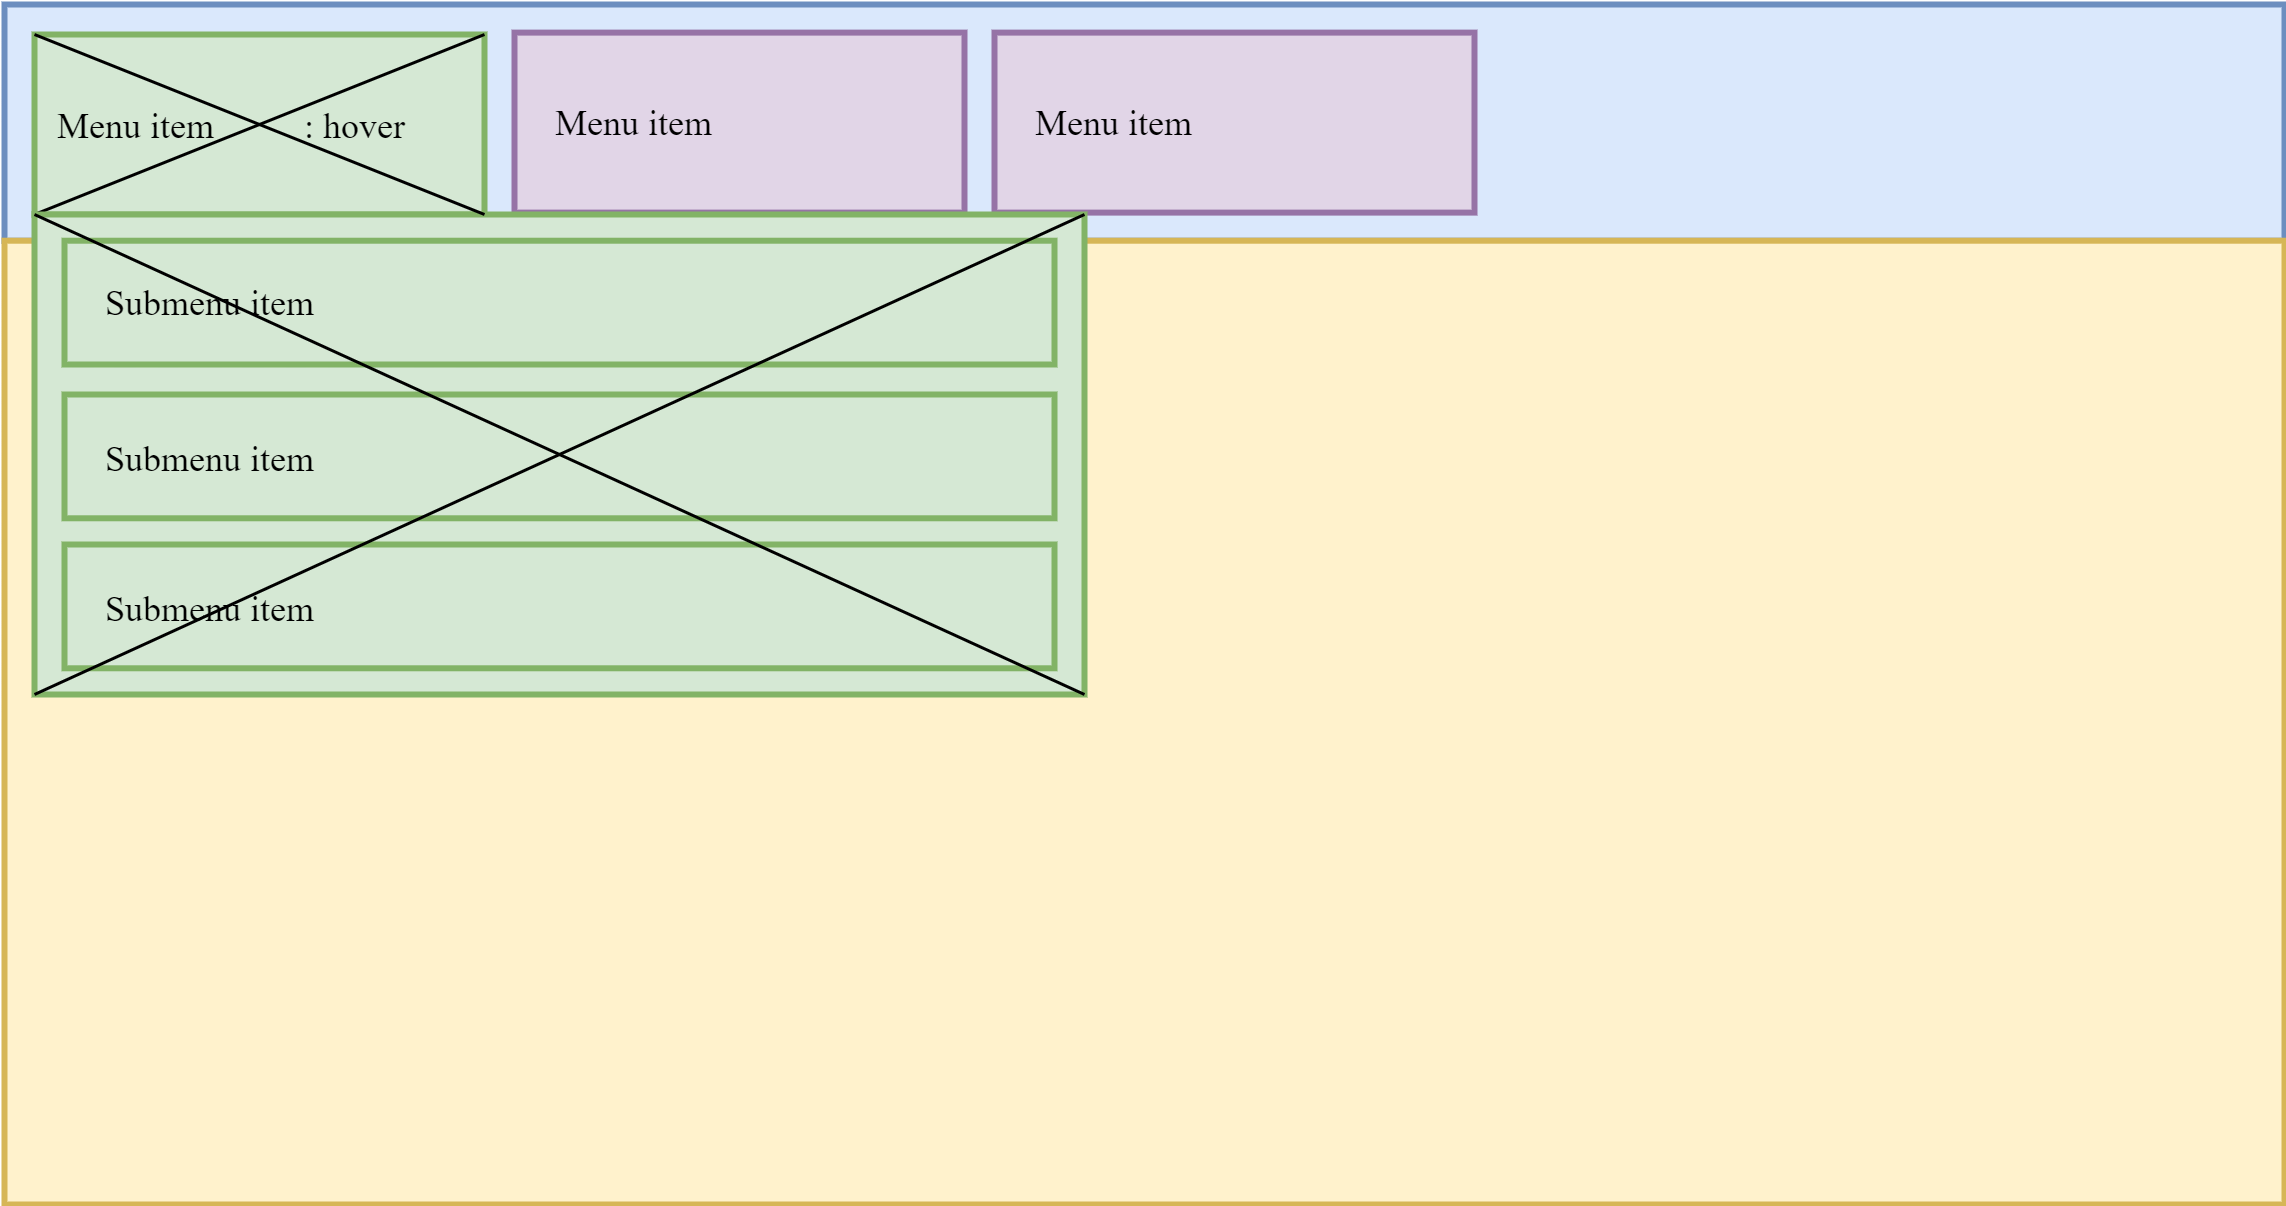
\includegraphics[width=12cm]
        {_assets/gpi_ui_menu.png}
    \caption{Макет мeню для компьютера}
    \label{fig:gpi_ui_menu}
\end{figure}

Макет страницы с таблицей для компьютера изображен на
\textbf{рис.~\ref{fig:gpi_ui_get}~(стр.~\pageref{fig:gpi_ui_get})}.

\begin{figure}[!hp]
    \centering
    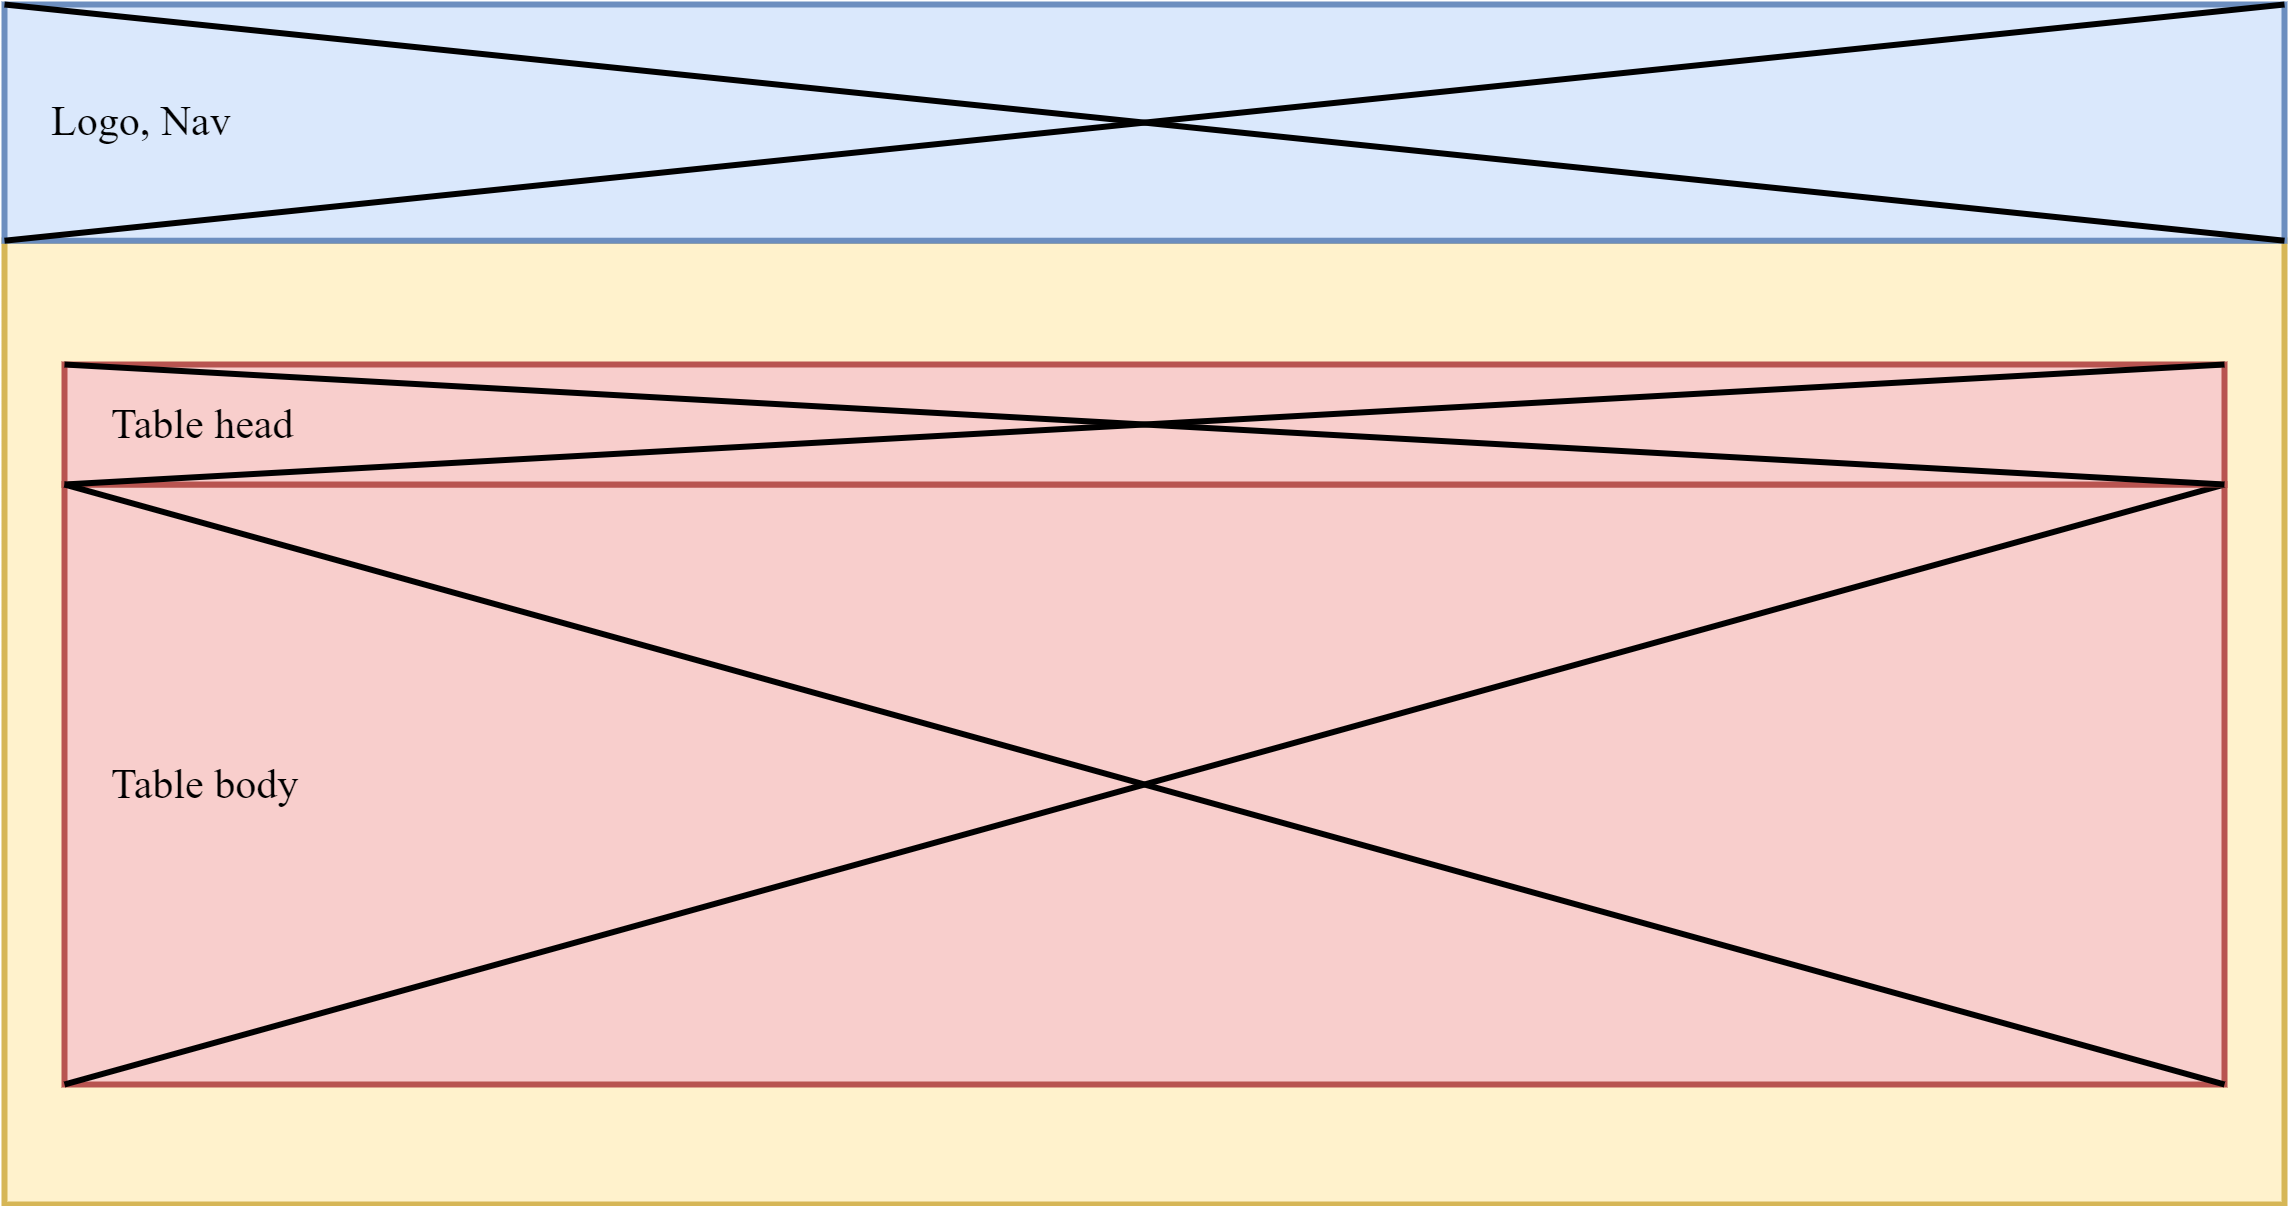
\includegraphics[width=12cm]
        {_assets/gpi_ui_get.png}
    \caption{Макет страницы с таблицей для компьютера}
    \label{fig:gpi_ui_get}
\end{figure}

Макет меню для телефона изображен на
\textbf{рис. \ref{fig:gpi_pz_phone_menu} (стр. \pageref{fig:gpi_pz_phone_menu})}.

\begin{figure}[!hp]
    \centering
    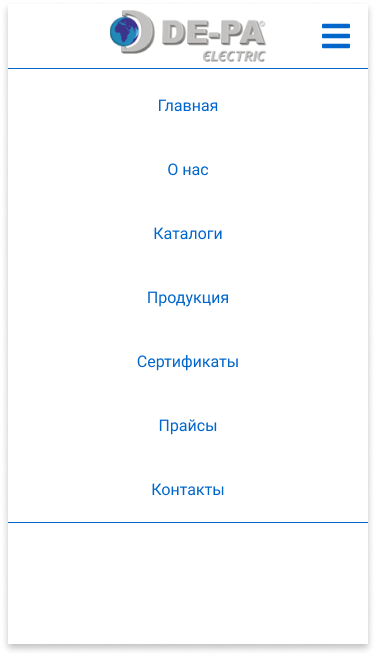
\includegraphics[height=16cm]
        {_assets/gpi_pz_android_menu.png}
    \caption{Макет меню для телефона}
    \label{fig:gpi_pz_phone_menu}
\end{figure}

\newpage

\subsection{Варианты использования программы в виде диаграмм прецедентов}

Первичное описание прецедентов для сотрудника изображено
на \textbf{рис.~\ref{fig:gpi_description_of_updated_use_case_employee} (стр.~\pageref{fig:gpi_description_of_updated_use_case_employee})}.

Первичное описание прецедентов для пользователя изображено
на \textbf{рис.~\ref{fig:gpi_description_of_updated_use_case_user} (стр.~\pageref{fig:gpi_description_of_updated_use_case_user})}.

\begin{figure}[!p]
    \centering
    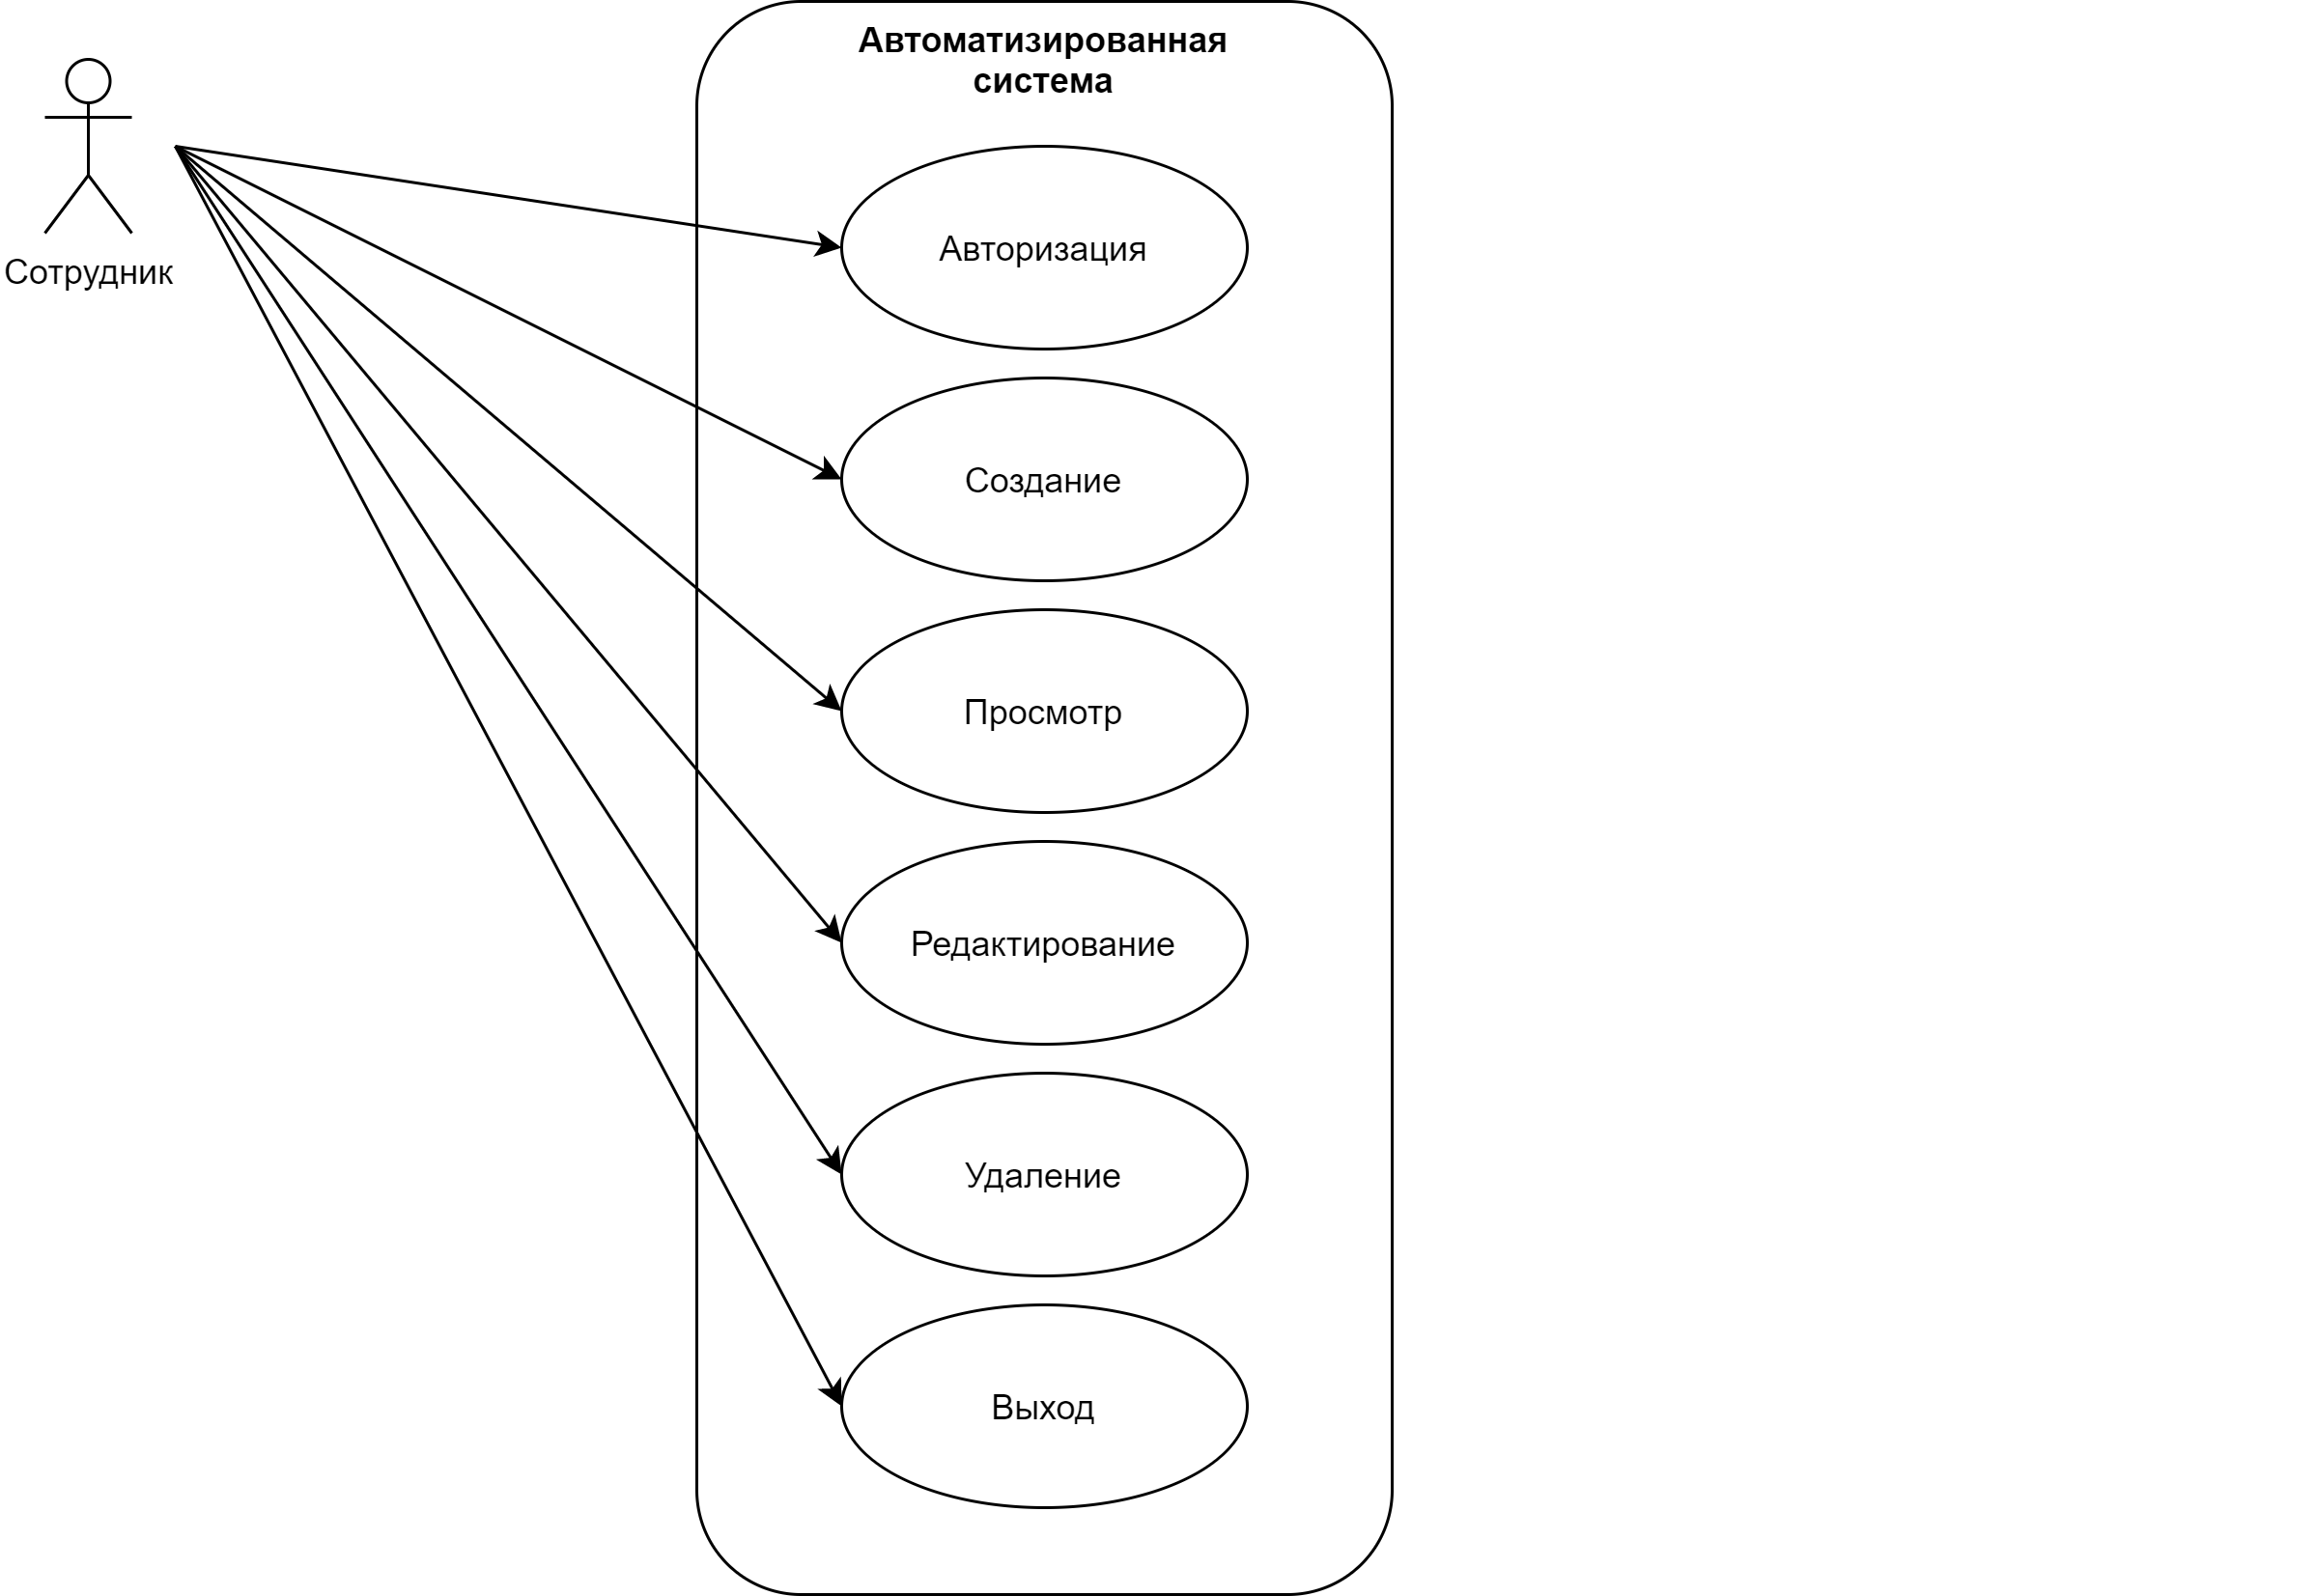
\includegraphics[width=14cm]
        {_assets/gpi_description_of_use_case_employee.png}
    \caption{Первичное описание прецедентов}
    \label{fig:gpi_description_of_updated_use_case_employee}
\end{figure}

\begin{figure}[!p]
    \centering
    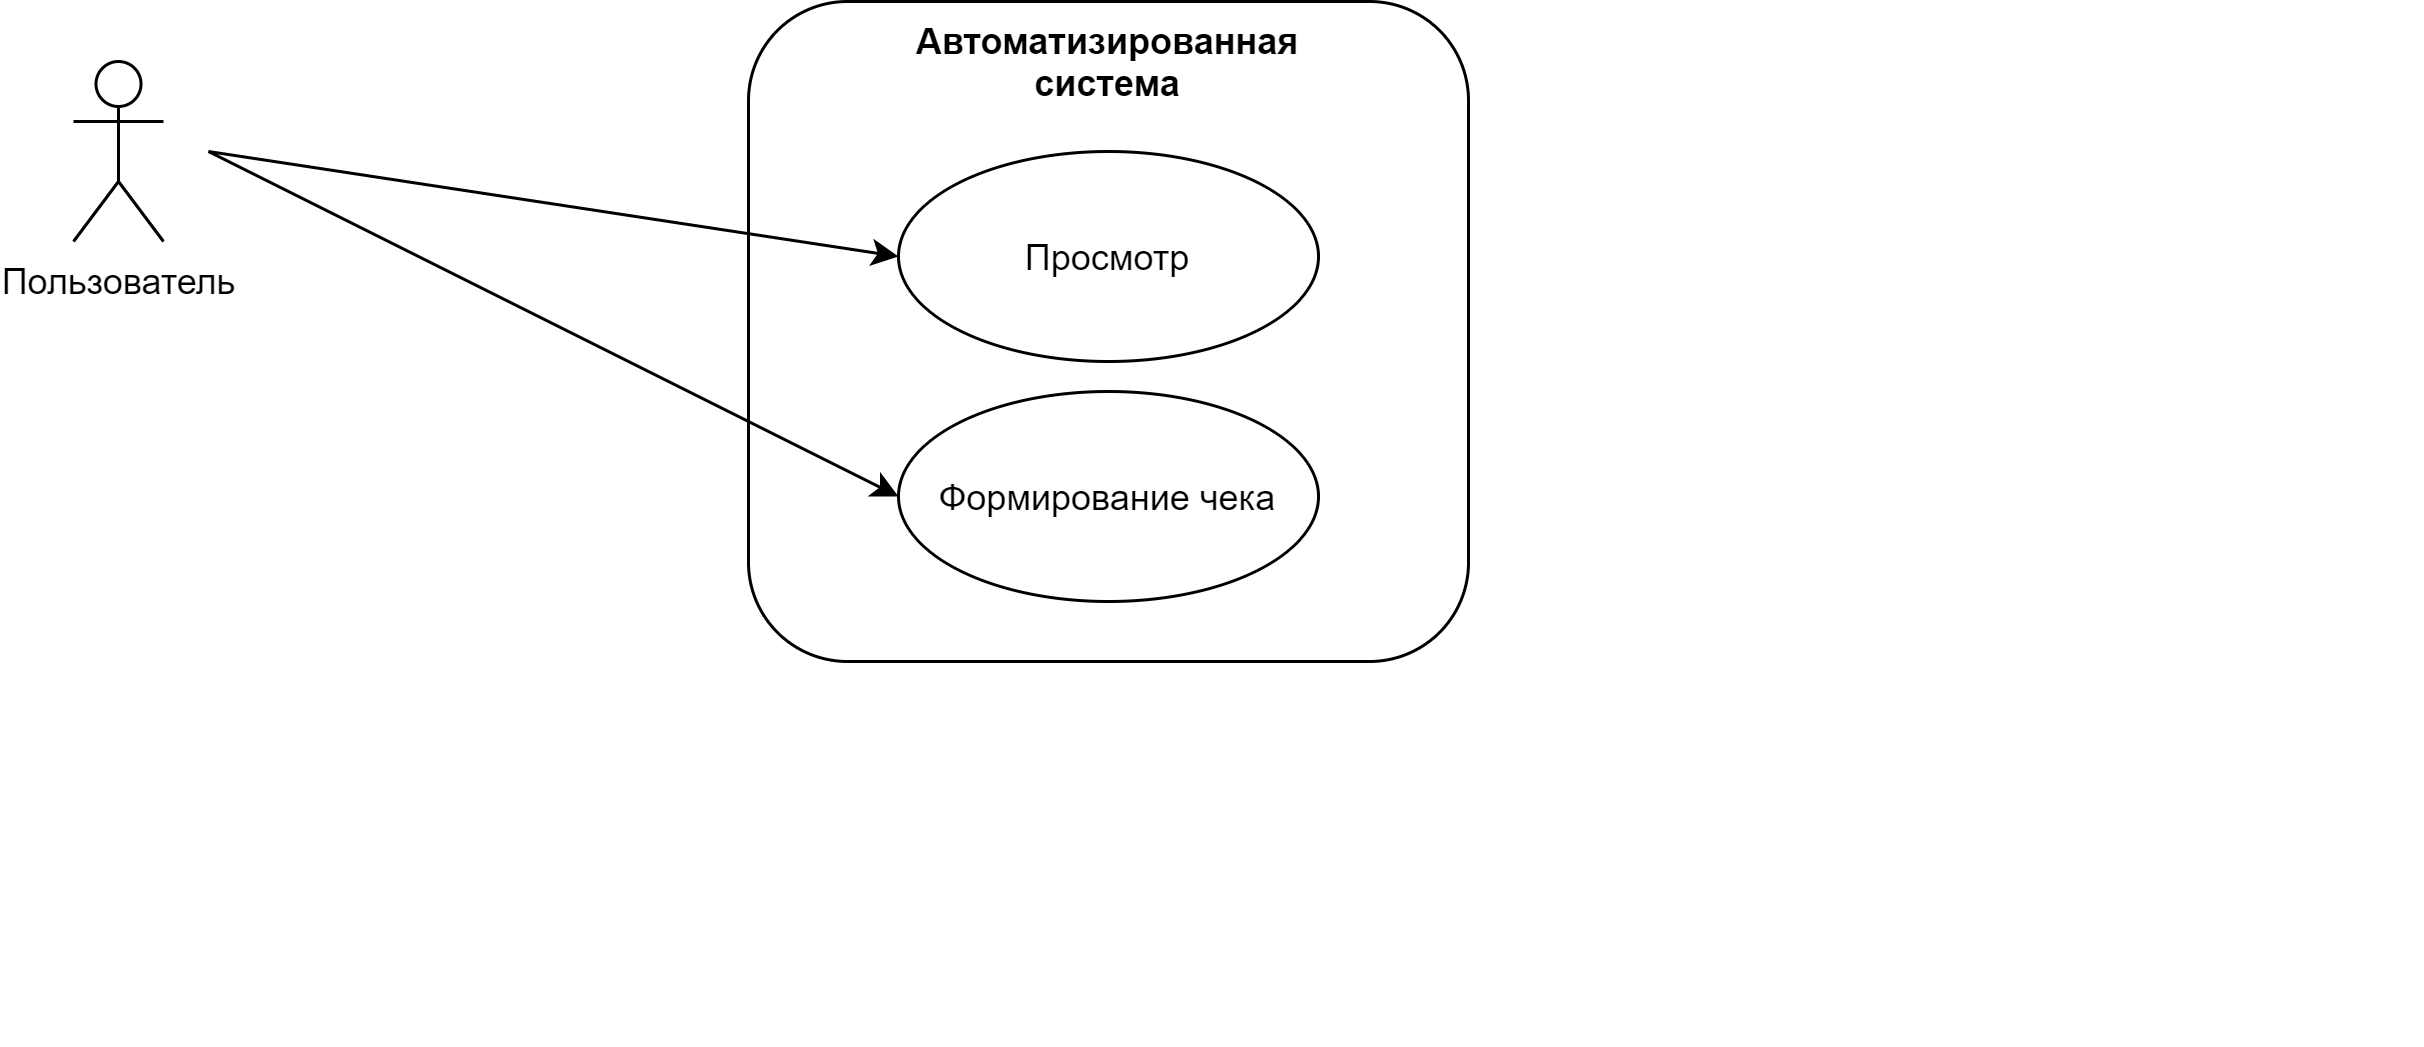
\includegraphics[width=14cm]
        {_assets/gpi_description_of_use_case_user.png}
    \caption{Первичное описание прецедентов}
    \label{fig:gpi_description_of_updated_use_case_user}
\end{figure}

\paragraph{Описание прецедентов:}

% = = = = = = = = = = = = = = = = = = = = = = = = = = = = = = = =

\subparagraph{\underline{Прецендент №1 <<Авторизация>>}} \hspace{0pt}

\textit{Назначение}: авторизация администратора.

\textit{Исполнители}: администратор, браузер.

\textit{Предусловие}: находимся на странице авторизации.

\textit{Основной поток событий}: администратор попадает в админ панель, иначе АПС.

\textit{Альтернативный поток событий}: сервер отошлет ответ, который не даст авторизоваться - и выдастся ошибка.

% = = = = = = = = = = = = = = = = = = = = = = = = = = = = = = = =

\subparagraph{\underline{Прецендент №2 <<Создание>>}} \hspace{0pt}

\textit{Назначение}: создание новой записи в БД.

\textit{Исполнители}: администратор, браузер.

\textit{Предусловие}: администратор авторизирован.

\textit{Основной поток событий}: В случае успешной авторизации администратора в БД добавится запись, иначе выполняется АПС.

\textit{Альтернативный поток событий}: администраторы прийдет ответ, который его выкинет на страницу авторизации.

% = = = = = = = = = = = = = = = = = = = = = = = = = = = = = = = =

\subparagraph{\underline{Прецендент №3 <<Просмотр>>}} \hspace{0pt}

\textit{Назначение}: просмотр справочника.

\textit{Исполнители}: администратор или пользователь, браузер.

\textit{Предусловие}: нет.

\textit{Основной поток событий}: получим массив записей, иначе выполняется АПС.

\textit{Альтернативный поток событий}: прийдет ответ об ошибке сервера.

% = = = = = = = = = = = = = = = = = = = = = = = = = = = = = = = =

\subparagraph{\underline{Прецендент №4 <<Редактирование>>}} \hspace{0pt}

\textit{Назначение}: редактирования записи в БД.

\textit{Исполнители}: администратор, браузер.

\textit{Предусловие}: администратор авторизирован.

\textit{Основной поток событий}: В случае успешной авторизации администратора в БД обновится запись, иначе выполняется АПС.

\textit{Альтернативный поток событий}: администраторы прийдет ответ, который его выкинет на страницу авторизации.

% = = = = = = = = = = = = = = = = = = = = = = = = = = = = = = = =

\subparagraph{\underline{Прецендент №5 <<Удаление>>}} \hspace{0pt}

\textit{Назначение}: удаление записи в БД.

\textit{Исполнители}: администратор, браузер.

\textit{Предусловие}: администратор авторизирован.

\textit{Основной поток событий}: В случае успешной авторизации администратора и подтверждения удаления в БД удалится запись, иначе выполняется АПС.

\textit{Альтернативный поток событий}: администраторы прийдет ответ, который его выкинет на страницу авторизации, либо пользователь отменит подтверждение удаления.

% = = = = = = = = = = = = = = = = = = = = = = = = = = = = = = = =

\subparagraph{\underline{Прецендент №6 <<Выход>>}} \hspace{0pt}

\textit{Назначение}: выход на страницу авторизации.

\textit{Исполнители}: администратор, браузер.

\textit{Предусловие}: пришёл ответ от сервера или администратор сам вышел.

\textit{Основной поток событий}: администратор окажется на странице авторизации.

% = = = = = = = = = = = = = = = = = = = = = = = = = = = = = = = =

\subparagraph{\underline{Прецендент №7 <<Формирование чека>>}} \hspace{0pt}

\textit{Назначение}: скачивание чека.

\textit{Исполнители}: пользователь, браузер.

\textit{Предусловие}: корзина не пуста.

\textit{Основной поток событий}: скачается чек, иначе выполняется АПС.

\textit{Альтернативный поток событий}: прийдет сообщение, что в корзине нет товаров.

% = = = = = = = = = = = = = = = = = = = = = = = = = = = = = = = =

\paragraph{Уточнённая диаграмма прецедентов} \hspace{0pt}

Уточнённая диаграмма прецедентов для сотрудника изображена
на \textbf{рис.~\ref{fig:gpi_description_of_updated_use_case_employee} (стр.~\pageref{fig:gpi_description_of_updated_use_case_employee})}.

Уточнённая диаграмма прецедентов для обычного пользователя изображена
на \textbf{рис.~\ref{fig:gpi_description_of_updated_use_case_user} (стр.~\pageref{fig:gpi_description_of_updated_use_case_user})}.

\begin{figure}[!p]
    \centering
    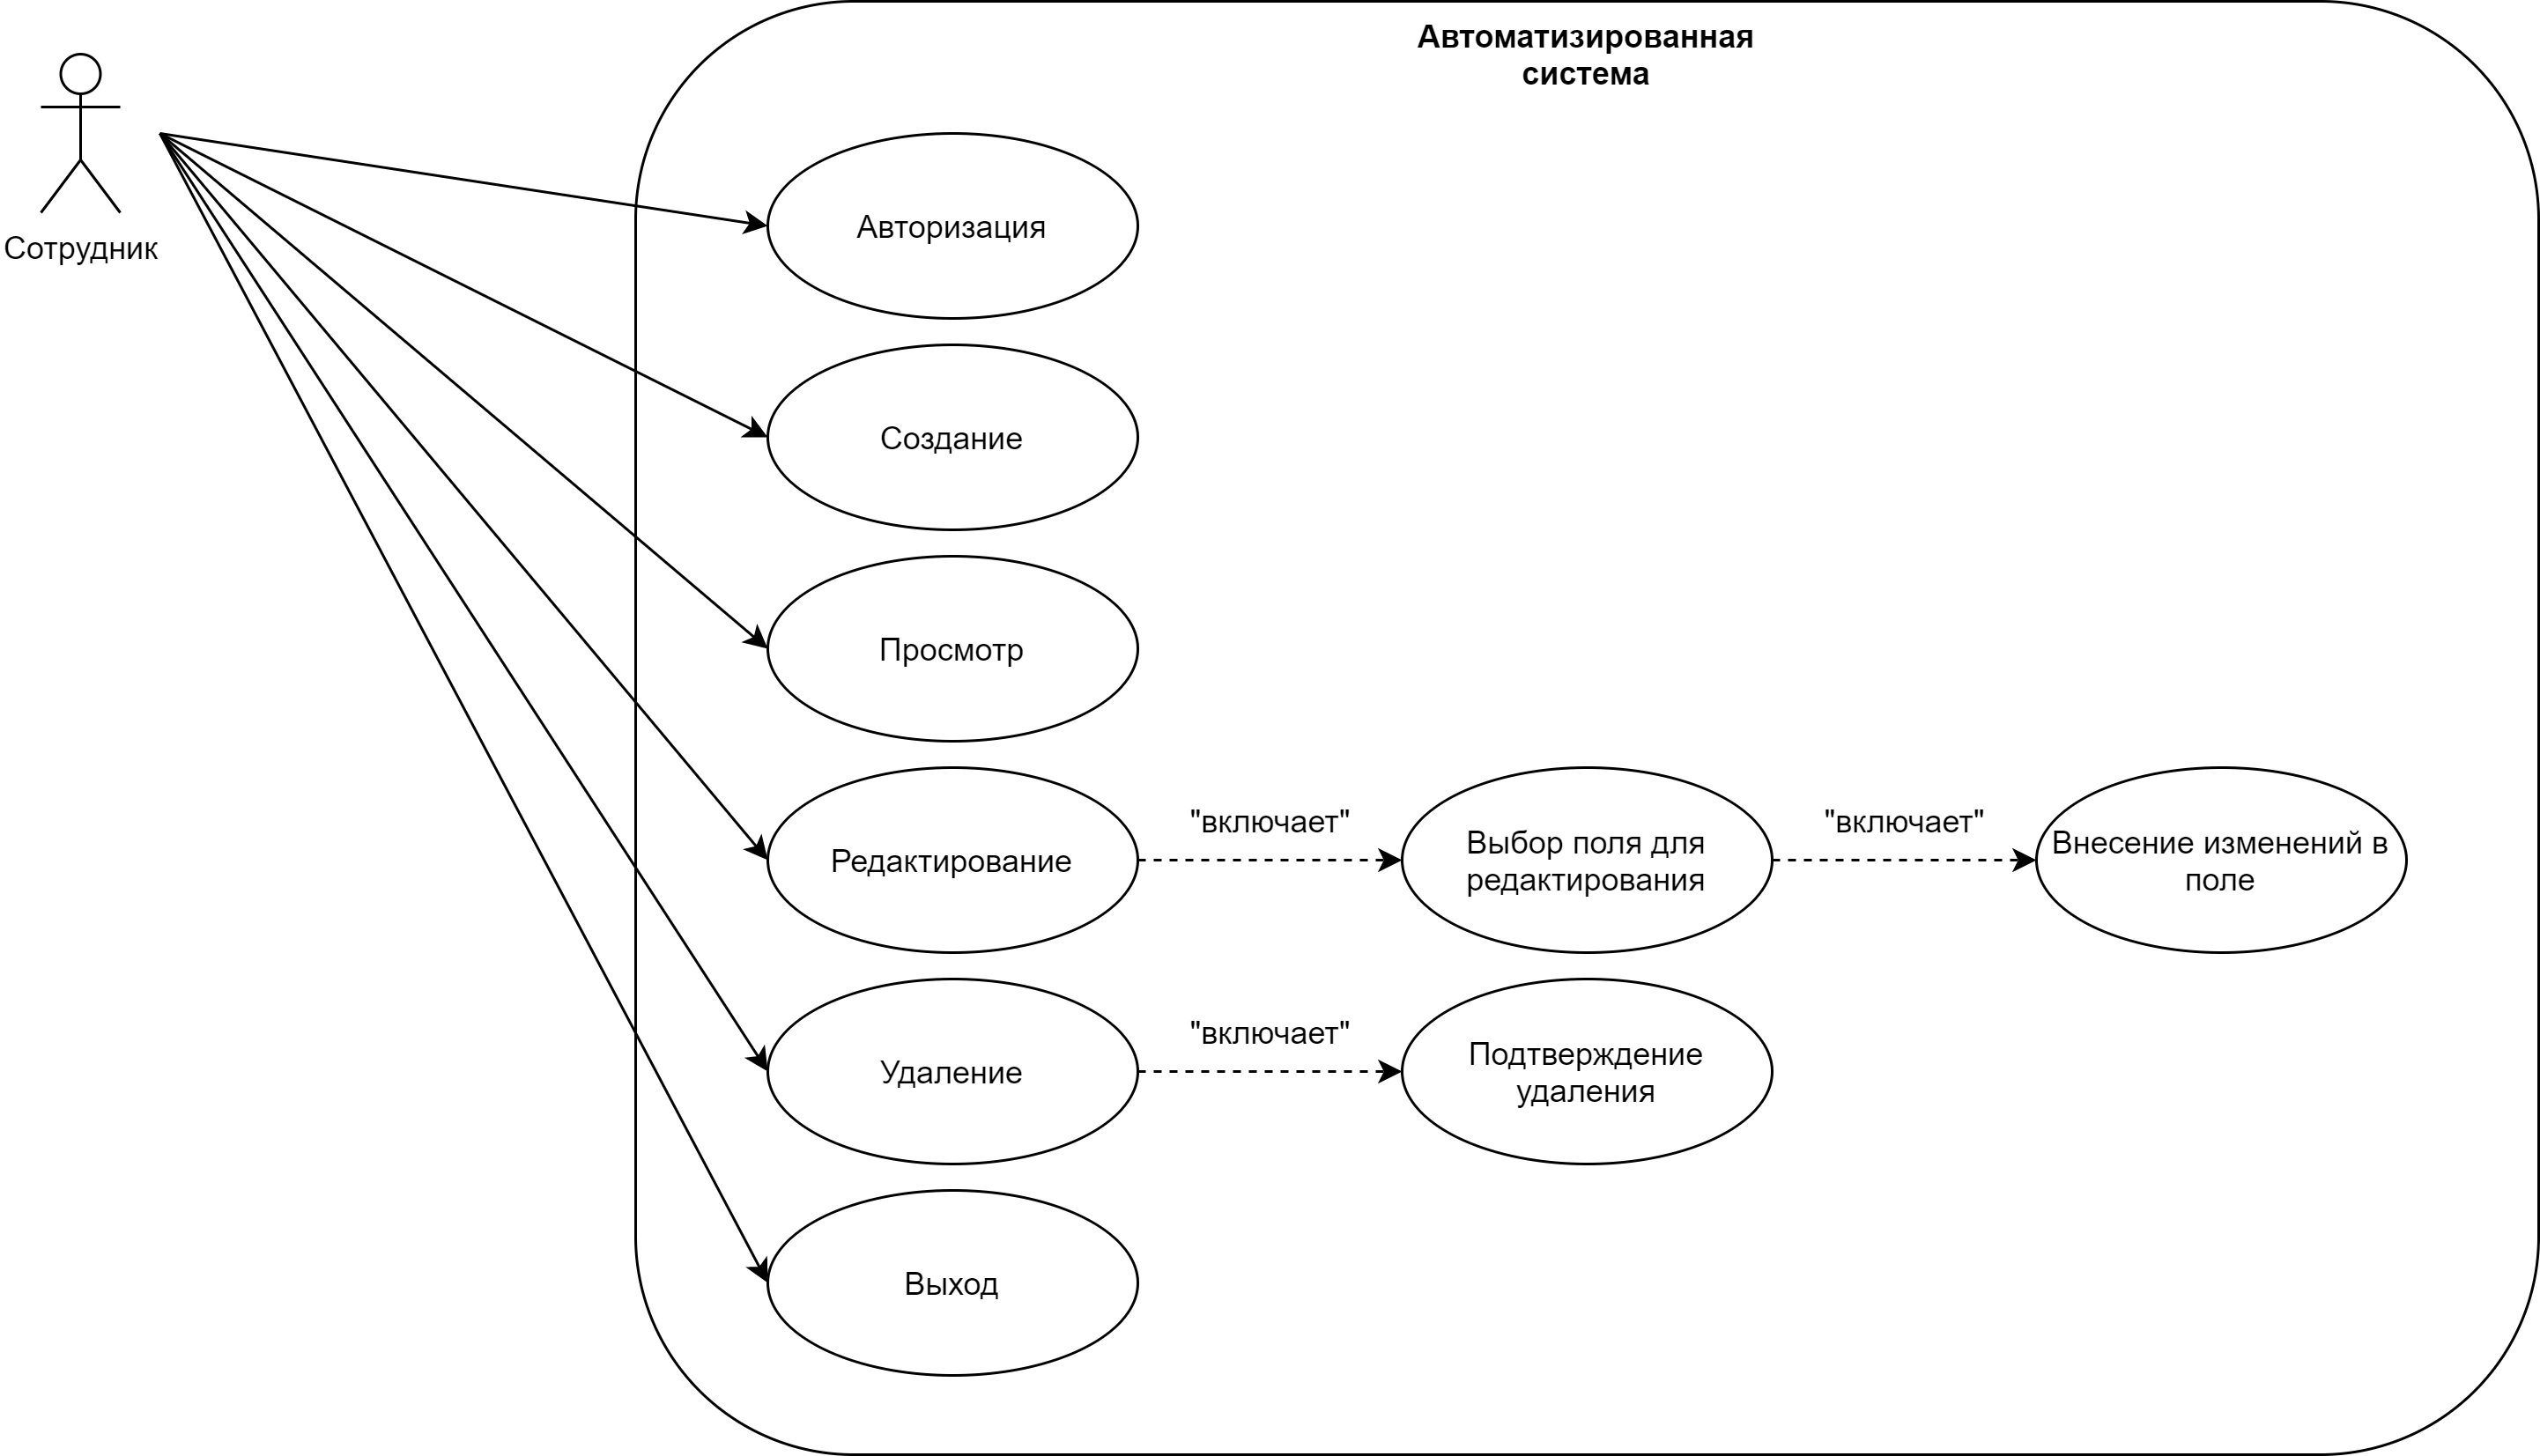
\includegraphics[width=14cm]
        {_assets/gpi_description_of_updated_use_case_employee.png}
    \caption{Первичное описание прецедентов}
    \label{fig:gpi_description_of_updated_use_case_employee}
\end{figure}

\begin{figure}[!p]
    \centering
    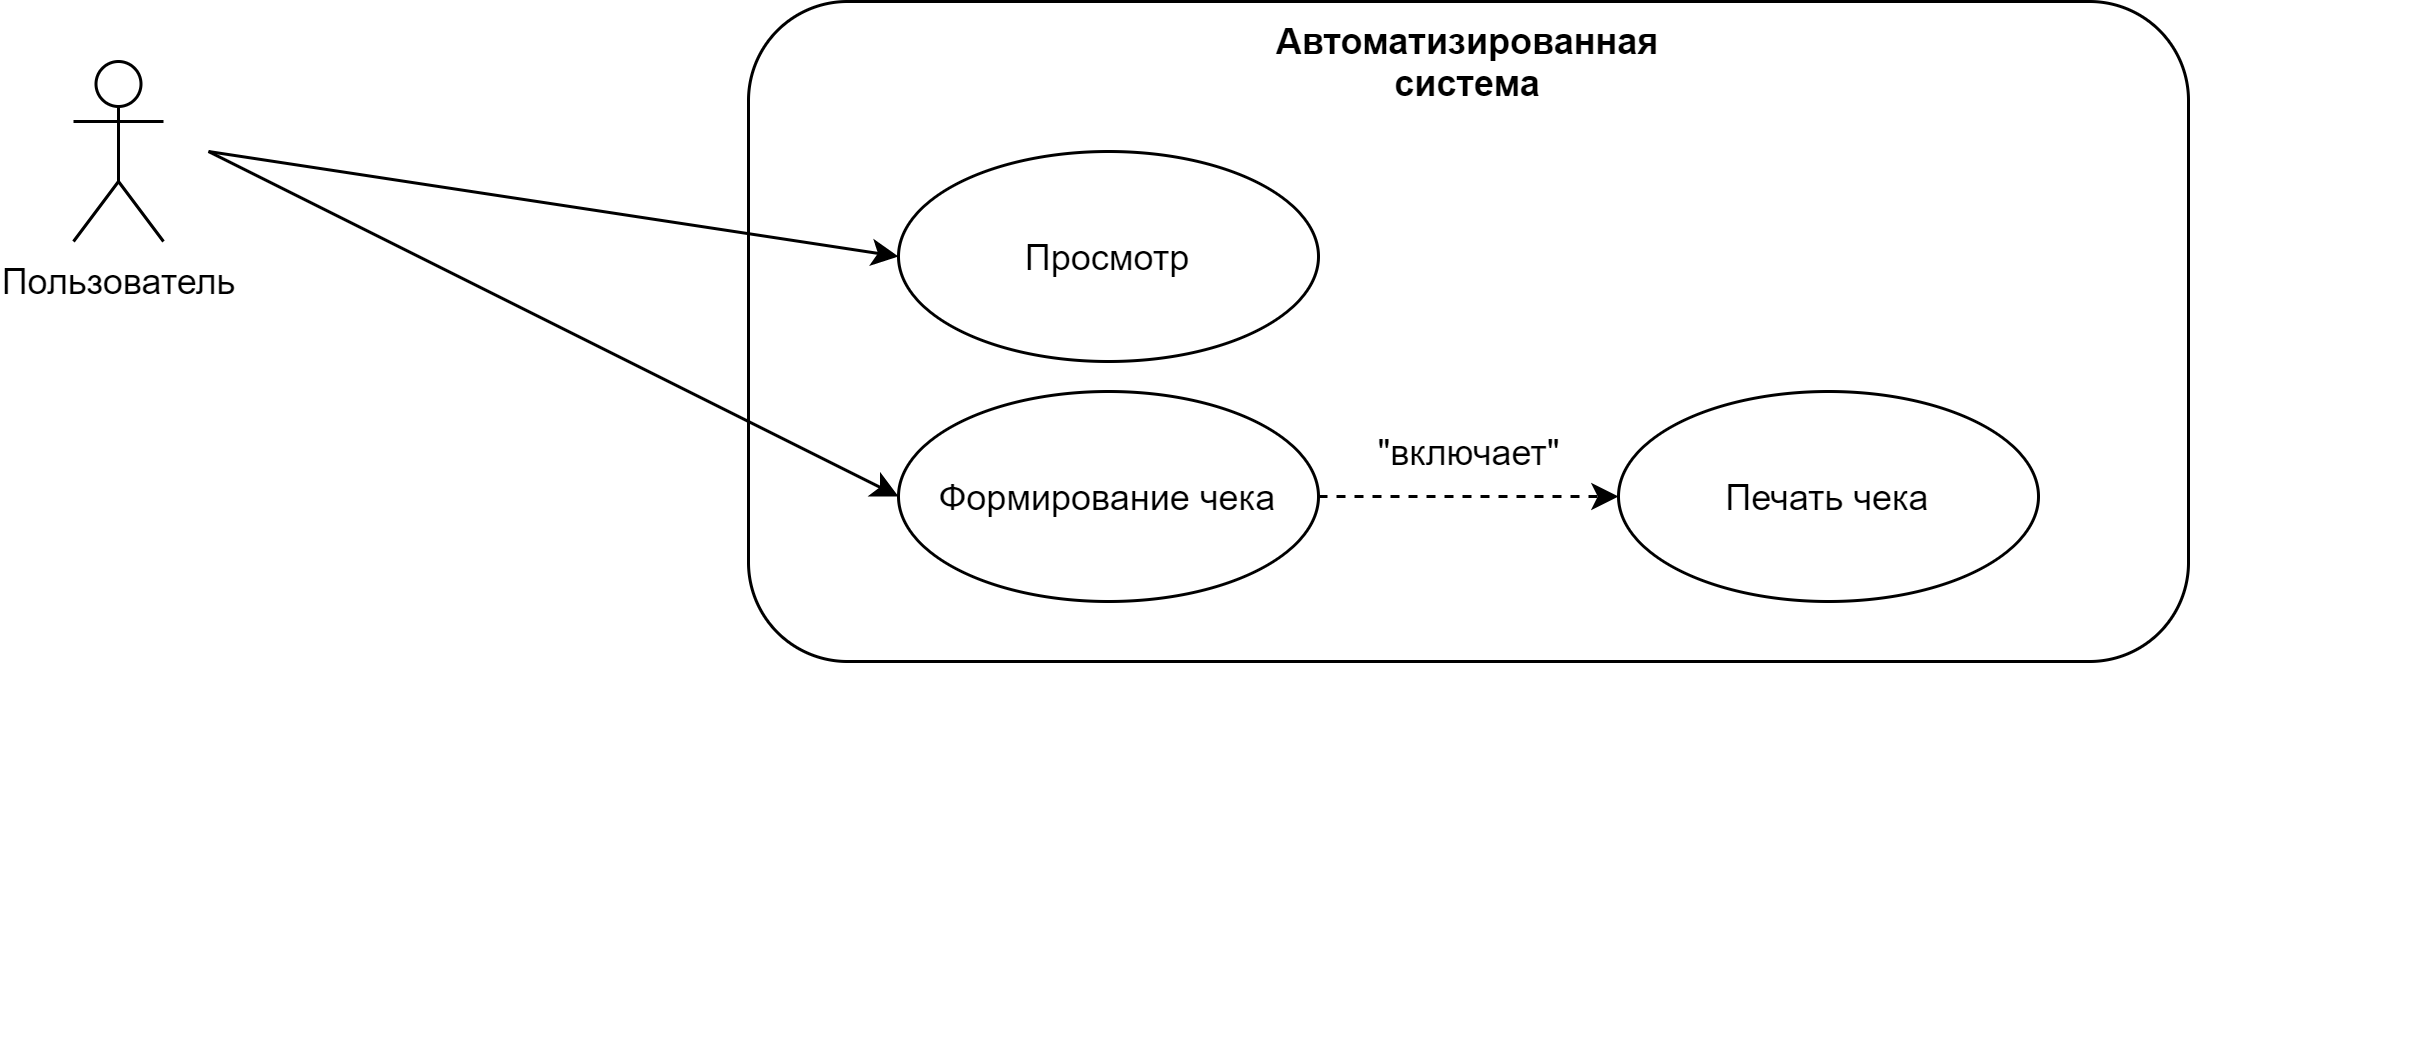
\includegraphics[width=14cm]
        {_assets/gpi_description_of_updated_use_case_user.png}
    \caption{Первичное описание прецедентов}
    \label{fig:gpi_description_of_updated_use_case_user}
\end{figure}

\newpage

\subsection{Первичное описание объектов и классов, прецедентов системы}

\paragraph{Описание классов} \hspace{0pt}

\textbf{Продукт} - класс, хранящий ифнормацию о продукте.

Свойства:
\begin{itemize}
    \item Model - модель товара.
    \item Name - наименование товара.
    \item CostBYN - цена за одну штуку без НДС в белорусских рублях.
    \item OnBox - количество в коробке.
    \item KG - вес коробки.
    \item M3 - размер коробки.
    \item Img - путь до картинки.
\end{itemize}

\textbf{Продукт} - класс, хранящий ифнормацию о блоке контакта.

Свойства:
\begin{itemize}
    \item title - заголовок контакта.
    \item description - описание контакта.
    \item phone1, phone2 - номер телефона.
    \item phone1Title, phone2Title - отображние номера телефона
    \item email1, email2 - электронная почта.
    \item viber - номер в Viber.
    \item whatsapp - номер в Whats App.
    \item skype - логин в Скайп.
    \item telegram - логин в Telegram.
\end{itemize}

\textbf{PDF} - класс, хранящий ифнормацию о прикрепленном файле.

Свойства:
\begin{itemize}
    \item Category - категория страницы.
    \item title - название документа, которое отображается на сайте.
    \item url - путь до PDF файла.
\end{itemize}

\paragraph{Диаграммы классов} \hspace{0pt}

Диаграмма класса Продукты изображена
на \textbf{рис.~\ref{fig:gpi_pz_product} (стр.~\pageref{fig:gpi_pz_product})}.

Диаграмма класса Контакты изображена
на \textbf{рис.~\ref{fig:gpi_pz_contacts} (стр.~\pageref{fig:gpi_pz_contacts})}.

Диаграмма класса PDF изображена
на \textbf{рис.~\ref{fig:gpi_pz_pdf} (стр.~\pageref{fig:gpi_pz_pdf})}.

\begin{figure}[!hb]
    \centering
    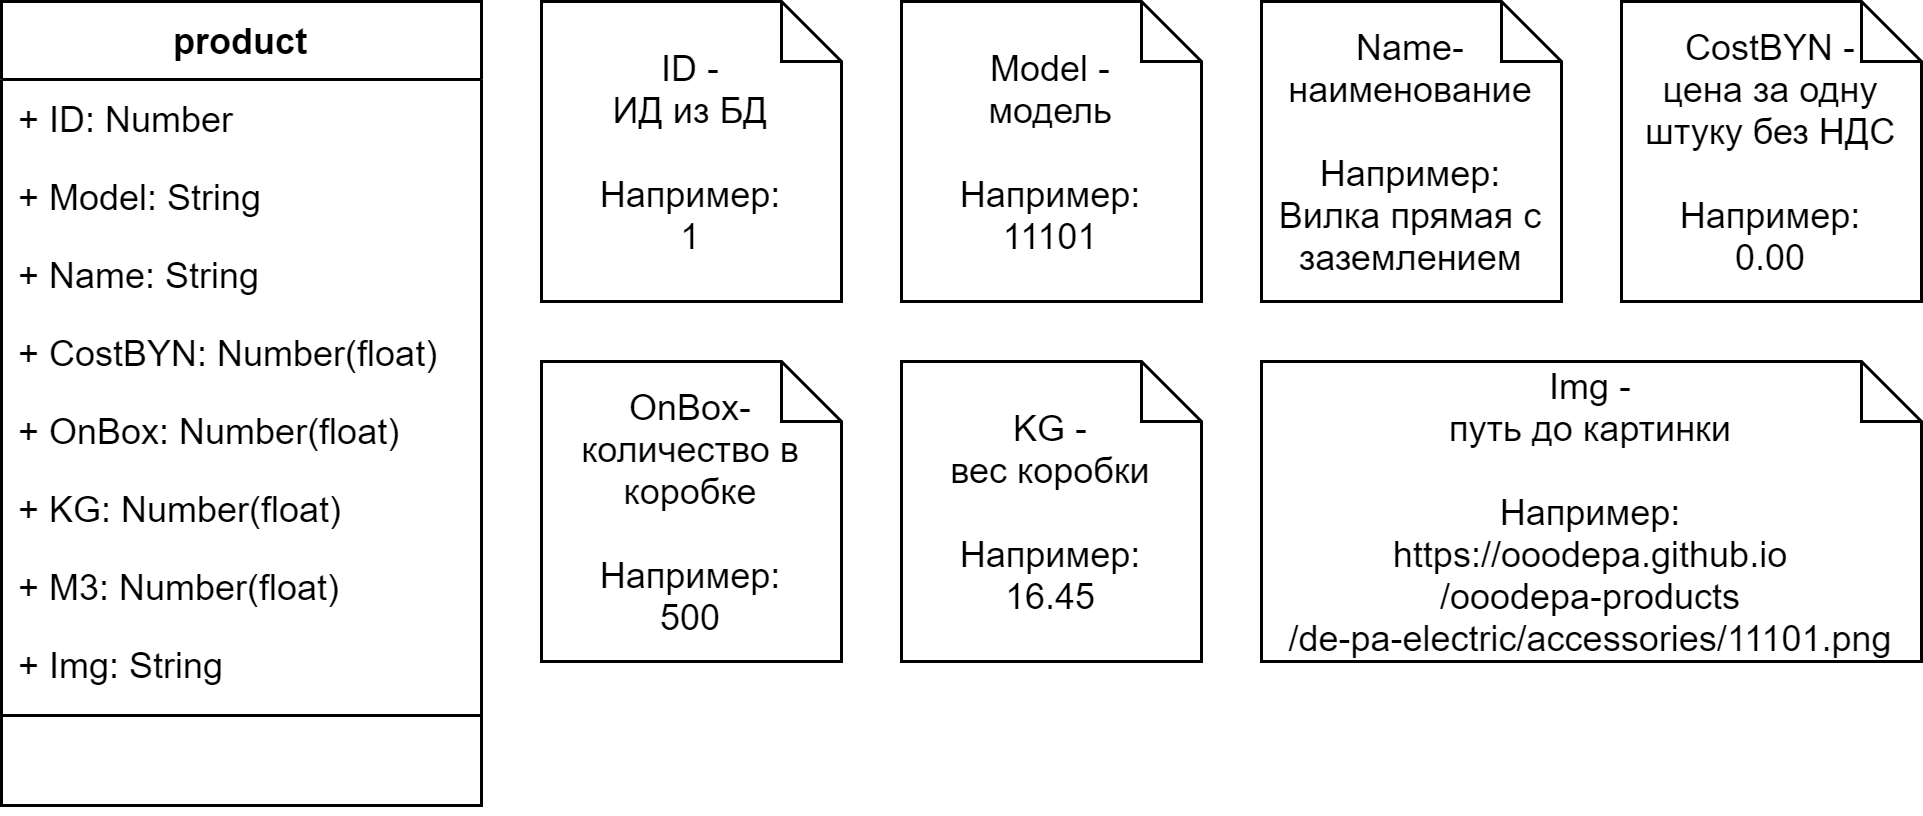
\includegraphics[width=12cm]
        {_assets/gpi_a_product.png}
    \caption{Диаграмма класса Продукты}
    \label{fig:gpi_pz_product}
\end{figure}

\begin{figure}[!hb]
    \centering
    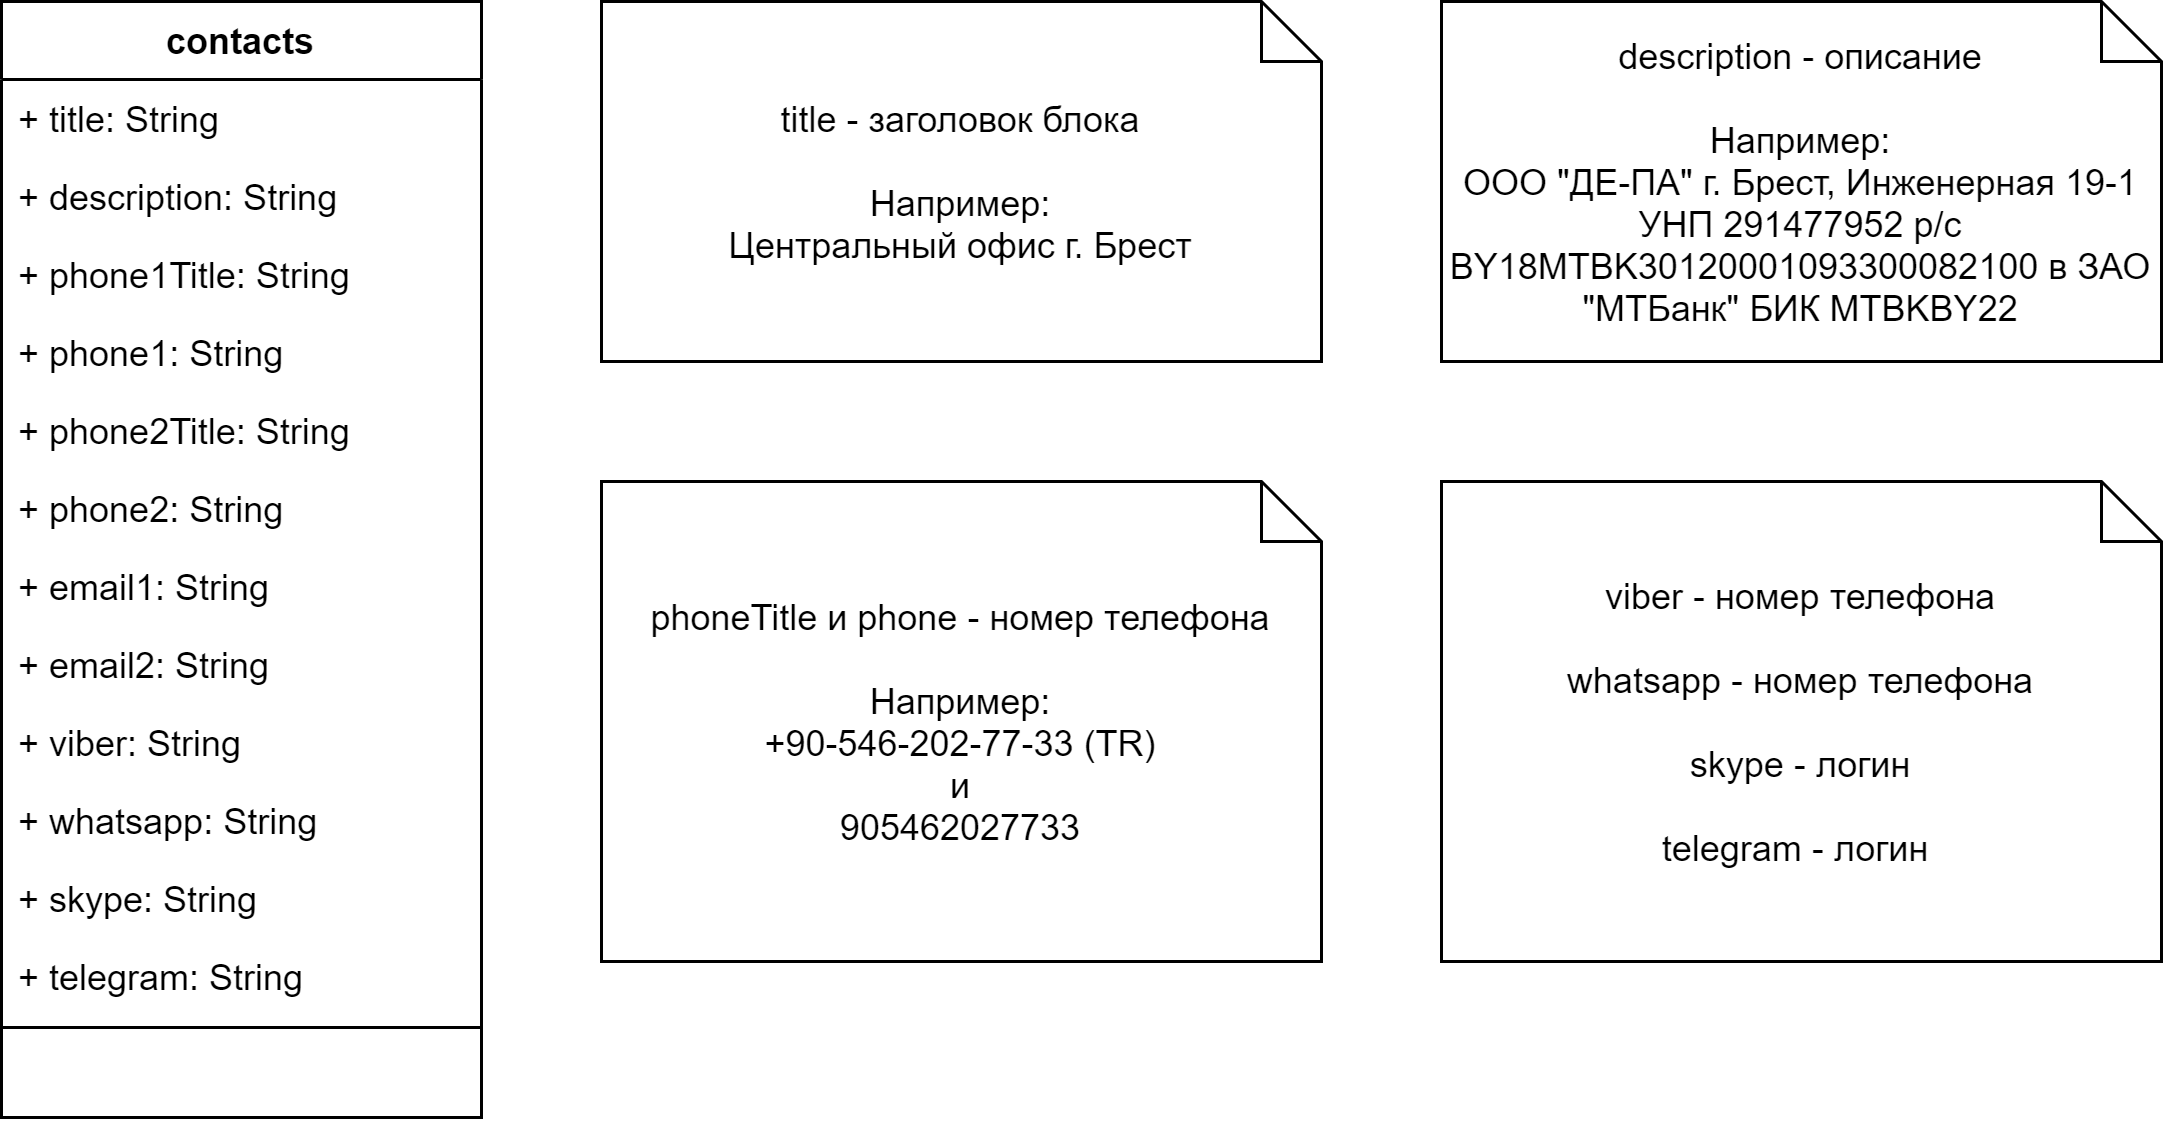
\includegraphics[width=12cm]
        {_assets/gpi_a_contacts.png}
    \caption{Диаграмма класса Контакты}
    \label{fig:gpi_pz_contacts}
\end{figure}

\begin{figure}[!hb]
    \centering
    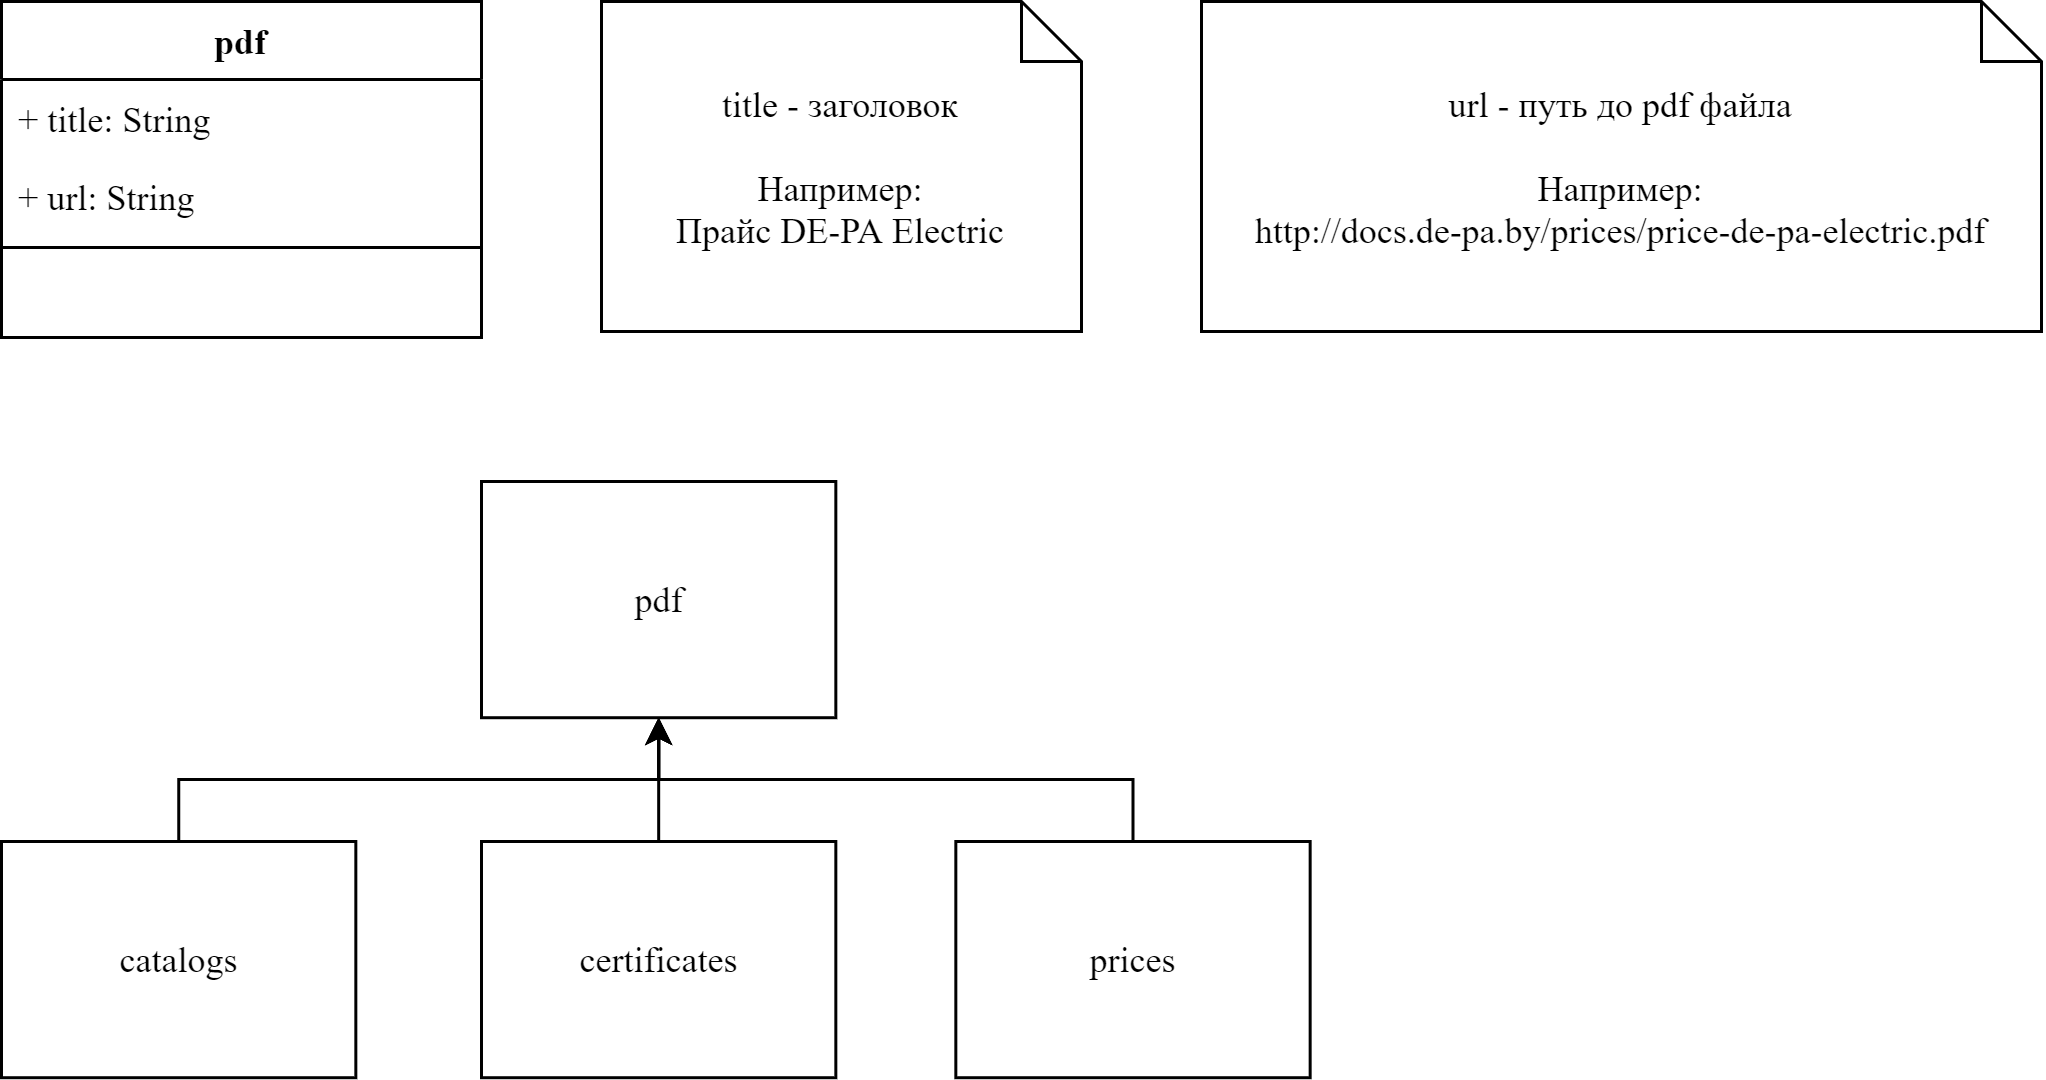
\includegraphics[width=12cm]
        {_assets/gpi_a_pdf.png}
    \caption{Диаграмма класса PDF}
    \label{fig:gpi_pz_pdf}
\end{figure}

\subsection{Проект. Схема данных}

Трёхуровневая архитектура - архитектурная модель программного комплекса,
предполагающая наличие в нём трёх компонентов: клиента, сервера приложений
(к которому подключено клиентское приложение) и сервера баз данных.

Если мы посмотрим на данную архитектуру с позиции сайта.
То первый уровень можно считать браузером (frontend), с помощью которого посетитель заходит на сайт,
второй уровень - это Express server (backend), а третий уровень - это база данных MySQL.

Схема архитуктуры ПО изображена на
\textbf{рис. \ref{fig:gpi_client_server} (стр. \pageref{fig:gpi_client_server})}.

\begin{figure}[!hp]
    \centering
    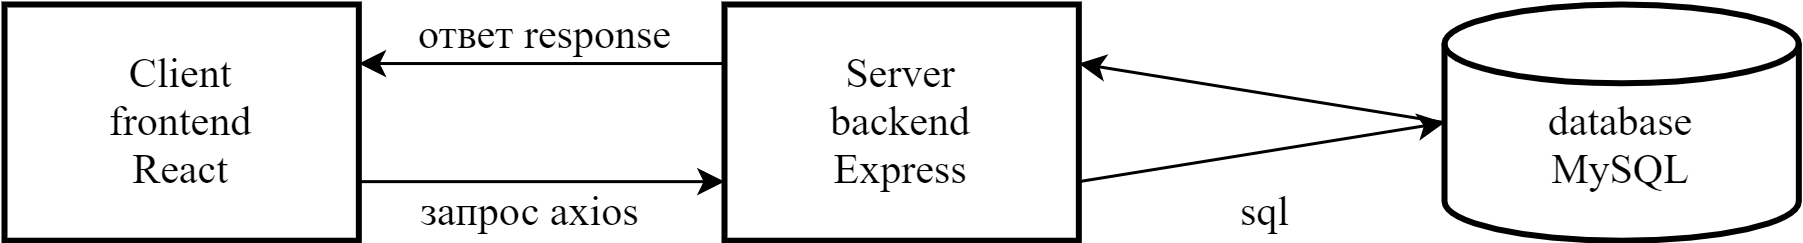
\includegraphics[width=16cm]
        {_assets/gpi_client_server.png}
    \caption{Схема архитектуры ПО}
    \label{fig:gpi_client_server}
\end{figure}

\newpage